% Drawing 79/06-2 -- folder 79, batch 06, archive page 111 (PDF page 112).
% Transcription: Un triangle de sommets $s_0$, $t_0$ (en bas) et $u_0$ (en haut), avec un petit secteur hachuré à partir de $s_0$, figurant la rotation autour de $s_0$.
% Kind: triangle with a hatched sector. Method 2 (schematic redraw from the facsimile). Status: ok.
% Notes: Triangle s_0 (left), t_0 (bottom right), u_0 (top); a small hatched sector at s_0 (a smaller triangle along the base), the rotation about s_0. The labels s_0 and t_0 are small; s_0 is at the left edge of the sheet's text and partly cut.
% Coordinates: 1 unit = 1 mm = 1/100 of the crop width (bbox in page fractions: [0.72, 0.08, 0.88, 0.17]).
% Redrawn by Claude (claude-opus-5-5), issue #73, 2026-11-07; not checked by a human; not compiled (no TeX in the session).
% Rights: reproduces part of the work -- behind RENDER_TRANSCRIPTS, never published by itself.
\documentclass[tikz,border=3pt]{standalone}
\usepackage{amsmath,amssymb}
\usetikzlibrary{patterns,arrows.meta}
\tikzset{pencil/.style={black!45}, struck/.style={black!35}, mark/.style={circle,draw,inner sep=1.3pt}, pt/.style={circle,fill,inner sep=0.9pt}, opt/.style={circle,draw,fill=white,inner sep=1.1pt}}
\begin{document}
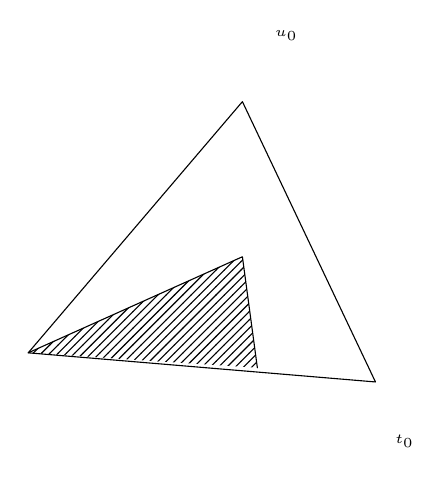
\begin{tikzpicture}[x=1mm,y=1mm,line cap=round,line join=round,font=\scriptsize]
\draw (34.4,-15) -- (7.2,-46.9) -- (51.3,-50.6) -- cycle;
\draw (7.2,-46.9) -- (34.4,-34.7) -- (36.3,-48.8);
\fill[pattern=north east lines] (7.2,-46.9) -- (34.4,-34.7) -- (36.3,-48.8) -- cycle;
\node[inner sep=1pt] at (40,-6.6) {\tiny $u_0$};
\node[inner sep=1pt] at (55,-58.1) {\tiny $t_0$};
\end{tikzpicture}
\end{document}
